\documentclass[12pt]{article}\usepackage[]{graphicx}\usepackage[]{color}
% maxwidth is the original width if it is less than linewidth
% otherwise use linewidth (to make sure the graphics do not exceed the margin)
\makeatletter
\def\maxwidth{ %
  \ifdim\Gin@nat@width>\linewidth
    \linewidth
  \else
    \Gin@nat@width
  \fi
}
\makeatother

\definecolor{fgcolor}{rgb}{0.345, 0.345, 0.345}
\newcommand{\hlnum}[1]{\textcolor[rgb]{0.686,0.059,0.569}{#1}}%
\newcommand{\hlstr}[1]{\textcolor[rgb]{0.192,0.494,0.8}{#1}}%
\newcommand{\hlcom}[1]{\textcolor[rgb]{0.678,0.584,0.686}{\textit{#1}}}%
\newcommand{\hlopt}[1]{\textcolor[rgb]{0,0,0}{#1}}%
\newcommand{\hlstd}[1]{\textcolor[rgb]{0.345,0.345,0.345}{#1}}%
\newcommand{\hlkwa}[1]{\textcolor[rgb]{0.161,0.373,0.58}{\textbf{#1}}}%
\newcommand{\hlkwb}[1]{\textcolor[rgb]{0.69,0.353,0.396}{#1}}%
\newcommand{\hlkwc}[1]{\textcolor[rgb]{0.333,0.667,0.333}{#1}}%
\newcommand{\hlkwd}[1]{\textcolor[rgb]{0.737,0.353,0.396}{\textbf{#1}}}%
\let\hlipl\hlkwb

\usepackage{framed}
\makeatletter
\newenvironment{kframe}{%
 \def\at@end@of@kframe{}%
 \ifinner\ifhmode%
  \def\at@end@of@kframe{\end{minipage}}%
  \begin{minipage}{\columnwidth}%
 \fi\fi%
 \def\FrameCommand##1{\hskip\@totalleftmargin \hskip-\fboxsep
 \colorbox{shadecolor}{##1}\hskip-\fboxsep
     % There is no \\@totalrightmargin, so:
     \hskip-\linewidth \hskip-\@totalleftmargin \hskip\columnwidth}%
 \MakeFramed {\advance\hsize-\width
   \@totalleftmargin\z@ \linewidth\hsize
   \@setminipage}}%
 {\par\unskip\endMakeFramed%
 \at@end@of@kframe}
\makeatother

\definecolor{shadecolor}{rgb}{.97, .97, .97}
\definecolor{messagecolor}{rgb}{0, 0, 0}
\definecolor{warningcolor}{rgb}{1, 0, 1}
\definecolor{errorcolor}{rgb}{1, 0, 0}
\newenvironment{knitrout}{}{} % an empty environment to be redefined in TeX

\usepackage{alltt}

%\usepackage[roman]{../pres1}
%\usepackage[sans]{../pres1}

\usepackage[hmargin=1in,vmargin=1in]{geometry}
\usepackage{parskip}
\usepackage{hyperref}
\usepackage{graphicx}
\usepackage{color}
\hypersetup{pdfstartview=FitV,hidelinks}




\IfFileExists{upquote.sty}{\usepackage{upquote}}{}
\begin{document}

{
  \Large
  \centering
  Lab 8 Assignment --- Occupancy Models \\
  Due before your next lab \par
}

\vspace{10pt}

%% Answer each of the following questions and upload your answers to ELC
%% as a single Excel file. Be sure to show your calculations. Name the
%% file something like: \texttt{Chandler\_Richard-lab8.xlsx}. \\

Answer each of the following questions, and submit your answers by
uploading a single \textcolor{red}{WORD} file to ELC. Unlike previous labs,
copy and paste results from Excel and PRESENCE to the WORD file. You should also copy and paste entire screenshots to show the relevant output. Name
the file something like \texttt{Chandler-lab8.docx}.  


%\vspace{12pt}


\section*{Occupancy models in program PRESENCE}

\subsection*{\normalsize Preliminaries: Getting Data into Program PRESENCE}
\vspace{-10pt}
\begin{enumerate}
  \itemsep-6pt
  \item[(1)]  Open PRESENCE
  \item[(2)]  Go to \texttt{File > New Project}
  \item[(3)]  Select \texttt{Input Data Form}
  \item[(4)]  Specify the number of rows (sites), columns
    (occasions), and (for Exercise I) the number of site covariates. 
  \item[(5)]  Fill in the number of occasions per season
    (No. Occ/season). For Exercise II, this is the number of teams per
    year. 
  \item[(6)]  Copy and paste occupancy data from Excel into the
    PRESENCE spreadsheet. 
  \item[(7)]  If you have a site covariate, click the \texttt{Site
      Covars} tab and copy and paste the covariate values (and the
    covariate name in the first row) using the option \texttt{Edit > Paste
    w/covnames}.  
  \item[(8)]  Use \texttt{File > Save As} to save the project
    somewhere on your computer. Save it to \texttt{Documents} or
    another location that isn't restricted. Click \texttt{No} when it
    asks if you want to use the last column as frequencies. 
  \item[(9)]  Close the PRESENCE spreadsheet, and click \texttt{OK} on
    the project information window.  
\end{enumerate}


\begin{figure}[h!]
  \centering
  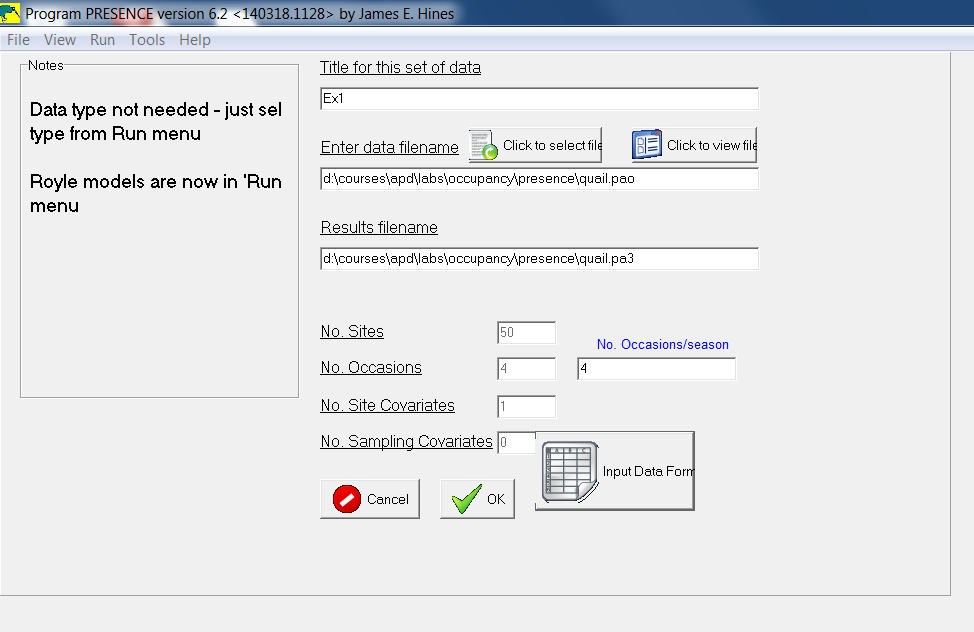
\includegraphics[width=0.7\textwidth]{figs/pres-setup}
  \caption{\small This is where you tell PRESENCE about your data}
  \label{fig:pres-setup}
\end{figure}

\clearpage

\subsection*{Exercise I: Single-season models}

Suppose we are interested in estimating occupancy of bobwhite quail
({\it Colinus virginianus}) in abandoned ag fields. We randomly select
50 sites and survey them 4 times each May. The resulting data indicate
whether at least one quail was detected at each site on each visit in
each season.    

In addition, you think there is a possibility that vegetation height
affects both occupancy and detection probability so you measure
average vegetation height at each site. Vegetation height will be the
covariate used in the analysis. 

Create a new PRESENCE project and import the quail data. You will
need to specify that there are 50 rows, 4 columns, 4 Occ/season, and 1
site covariate: \texttt{veght}. Make sure you use \texttt{Paste with
  covname} when adding the \texttt{veght} site covariate (see
instructions above).  

\begin{enumerate}
  \item[(a)] Run the single-season analysis without changing the
    defaults (\texttt{Run > Analysis:single-season}). Report the
    estimates and standard errors for psi ($\psi$) and p. Interpret
    these estimates (ie, what are the definitions of psi and p in this
    context?). These can be found by right-clicking on the name of the
    model (which will be something like \texttt{1 group, constant P}
    and clicking on \texttt{View model output}.  There is LOTS of
    output. You want to focus on the \texttt{Individual Site
      Estimates}, which should look something like this: 

\begin{figure}[h!]
  \centering
  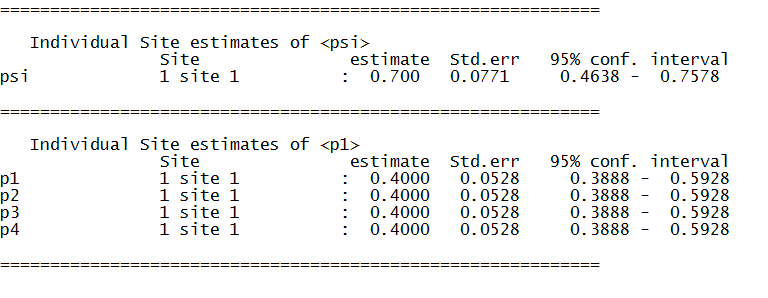
\includegraphics[width=0.9\textwidth]{figs/pres-est}
  \caption{\small Estimates, standard errors, and confidence intervals
  for psi ($\psi$) and $p$.}
  \label{fig:pres-est}
\end{figure}
    
  \item[(b)] Now run another model using \texttt{veght} as a
    predictor variable (covariate). This is tricky. First, choose 
    \texttt{Run > Analysis:single-season}. Then, click on
    \texttt{Custom}, which will open up the ``design matrix''. Now
    right click to \texttt{Add col} on the Occupancy tab (see
    Fig. below). Next, click the cell under \texttt{a2} and select 
    \texttt{Init > *veght} to indicate that you want to model psi
    as a function of vegetation height. Do the same thing under the
    \texttt{Detection} tab, but note that there are multiple rows for
    a1 and a2 this time. Make sure the first column of each matrix has
    1's not 0's (see screenshots below). Close the design matrix
    window and then name the model something like 
    \texttt{psi(veght)p(veght)} and hit \texttt{OK to Run}. 

\begin{figure}[h!]
  \centering
  \fbox{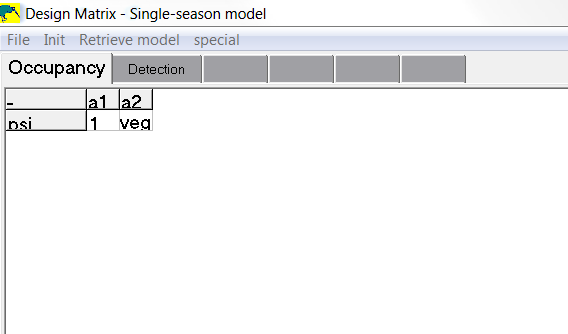
\includegraphics[height=5cm]{figs/pres-des-psi}} \hfill
  \fbox{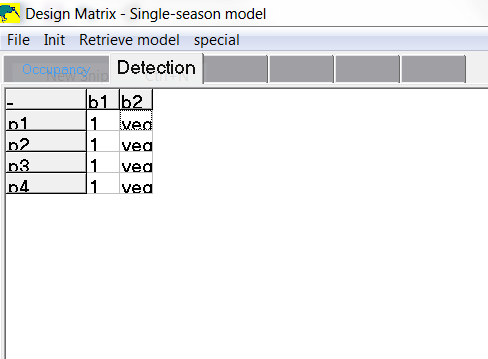
\includegraphics[height=5cm]{figs/pres-des-p}}   \\
  \caption{\small This is where you tell PRESENCE about the covariates
    in the model.}
  \label{fig:pres-design}
\end{figure}
%\clearpage

  \item[(c)] Is this model better than the first, based on AIC? The
    lower the AIC the better the model.\footnote{$\mathrm{AIC} =
      -2*\mathrm{log(likelihood)} + 2*\mathrm{nParameters}$. AIC
      favors models that explain a lot of variation in the data using
      a small number of parameters.}  
  \item[(d)] Right-click on the model and choose 
    \texttt{View model output} to find the parameter estimates under
    \texttt{Untransformed Estimates of coefficients for covariates
      (Beta's)}.  The estimate \texttt{A1} is the estimate of the
    intercept, and \texttt{A2} is the slope parameter defining the
    relationship between psi and vegetation height on the logit
    scale. Use these estimates to create a plot of the relationship
    between occurrence probability and vegetation height. The Excel
    sheet has a template for you to fill in. Add the graph to your
    Word document.
  \item[(e)] Based on your graph, does occurrence probability
    increase or decrease with vegetation height?  
\end{enumerate}

\clearpage

\subsection*{Exercise II: Multi-season model}

Use the southern two-lined salamander ({\it Eurycea cirrigera})
%Eastern newt ({\it Notophthalmus viridescens}) 
data from the
past few years to do the following. Note: I pooled the data from
the 5 swipes of each team.   

\begin{enumerate}
  \item[(a)] Close your old project, restart PRESENCE, and create a
    new project by importing the salamander
    data. You will need to indicate that there are 15 sites, 35
    columns, and \textcolor{red}{7 occasions per season}. The last piece of
    information tells PRESENCE that there were 5 seasons (with 7 team
    surveys per season).  
  \item[(b)] Use Program PRESENCE to estimate psi ($\psi$), gamma
    ($\gamma$), epsilon ($\epsilon$),
    and p (\texttt{Run > Analysis:multi-season > simple multi-season}
    and accept default settings). The estimates can be found by right clicking on the
    model name and choosing \texttt{View model output}. Look for the 
    \texttt{Real parameter estimates}. Report the 4 unique
    estimates and standard errors by creating a table in your Word
    document.  
  \item[(c)] Provide clear interpretations of your estimates. 
  \item[(d)] Based on these estimates, is there any reason to believe
    that occupancy has decreased over these years? Explain. 
  \item[(e)] How certain are you of these conclusions? Answer by
    describing how well you think our study design met the assumptions
    of the multi-season occupancy model. 

\end{enumerate}




\clearpage


\section*{Occupancy modeling in \texttt{R}}

\subsubsection*{Install the `unmarked' package}

Occupancy models can be fit using the `unmarked' package in {\tt R}. To install `unmarked', issue this command in R or RStudio:

\begin{knitrout}
\definecolor{shadecolor}{rgb}{0.969, 0.969, 0.969}\color{fgcolor}\begin{kframe}
\begin{alltt}
\hlkwd{install.packages}\hlstd{(}\hlstr{"unmarked"}\hlstd{)}
\end{alltt}
\end{kframe}
\end{knitrout}

Once it's installed, you need to load it:

\begin{knitrout}
\definecolor{shadecolor}{rgb}{0.969, 0.969, 0.969}\color{fgcolor}\begin{kframe}
\begin{alltt}
\hlkwd{library}\hlstd{(unmarked)}
\end{alltt}
\end{kframe}
\end{knitrout}

\section*{Import the data}

Now we're ready to import the data. The easiest way to do this is to save the data as a \texttt{.csv} file, and put it in your working directory. The working directory is the locatio on your computer where {\bf R} will look for files by default. To find out where the working directory is, do this:

\begin{knitrout}
\definecolor{shadecolor}{rgb}{0.969, 0.969, 0.969}\color{fgcolor}\begin{kframe}
\begin{alltt}
\hlkwd{getwd}\hlstd{()}
\end{alltt}
\begin{verbatim}
## [1] "c:/Users/RichardC/courses/applied-popdy/labs/occupancy-modeling"
\end{verbatim}
\end{kframe}
\end{knitrout}

If that is the location where your data are, you're ready to import. Otherwise, you need to change your working directory using the drop-down menu options, or using a command like:

\begin{knitrout}
\definecolor{shadecolor}{rgb}{0.969, 0.969, 0.969}\color{fgcolor}\begin{kframe}
\begin{alltt}
\hlkwd{setwd}\hlstd{(}\hlstr{"C:/Users/Richard/Documents/APD/"}\hlstd{)} \hlcom{## Modify the path in quotes}
\end{alltt}
\end{kframe}
\end{knitrout}

Once your working directory is correctly specified, you can import the data using this command:

\begin{knitrout}
\definecolor{shadecolor}{rgb}{0.969, 0.969, 0.969}\color{fgcolor}\begin{kframe}
\begin{alltt}
\hlstd{exampleData} \hlkwb{<-} \hlkwd{read.csv}\hlstd{(}\hlstr{"example-data.csv"}\hlstd{)}
\end{alltt}
\end{kframe}
\end{knitrout}

Let's look at a summary:

\begin{knitrout}\footnotesize
\definecolor{shadecolor}{rgb}{0.969, 0.969, 0.969}\color{fgcolor}\begin{kframe}
\begin{alltt}
\hlkwd{summary}\hlstd{(exampleData)}
\end{alltt}
\begin{verbatim}
##        X      season1visit1  season1visit2 season1visit3  season1visit4 
##  site1  : 1   Min.   :0.00   Min.   :0.0   Min.   :0.00   Min.   :0.00  
##  site10 : 1   1st Qu.:0.00   1st Qu.:0.0   1st Qu.:0.00   1st Qu.:0.00  
##  site11 : 1   Median :0.00   Median :0.0   Median :0.00   Median :0.00  
##  site12 : 1   Mean   :0.34   Mean   :0.3   Mean   :0.34   Mean   :0.28  
##  site13 : 1   3rd Qu.:1.00   3rd Qu.:1.0   3rd Qu.:1.00   3rd Qu.:1.00  
##  site14 : 1   Max.   :1.00   Max.   :1.0   Max.   :1.00   Max.   :1.00  
##  (Other):44                                                             
##   habitatIndex  
##  Min.   :1.040  
##  1st Qu.:1.925  
##  Median :3.135  
##  Mean   :3.021  
##  3rd Qu.:3.895  
##  Max.   :4.760  
## 
\end{verbatim}
\end{kframe}
\end{knitrout}

Columns 2-4 have the occupancy data. The fifth column has a site-specific covariate. Before we can run a single-season occupancy model, we have to format the data:


\section*{Format the data}



\begin{knitrout}
\definecolor{shadecolor}{rgb}{0.969, 0.969, 0.969}\color{fgcolor}\begin{kframe}
\begin{alltt}
\hlcom{## First, extract columns 2-4 with the occupancy data}
\hlstd{occData} \hlkwb{<-} \hlstd{exampleData[,}\hlkwd{c}\hlstd{(}\hlstr{"season1visit1"}\hlstd{,} \hlstr{"season1visit2"}\hlstd{,}
                          \hlstr{"season1visit2"}\hlstd{,} \hlstr{"season1visit4"}\hlstd{)]}
\hlcom{## Next, extract the column with the site covariate.}
\hlcom{## It must be formatted as a data.frame}
\hlstd{habIndex} \hlkwb{<-} \hlstd{exampleData[,}\hlkwd{c}\hlstd{(}\hlstr{"habitatIndex"}\hlstd{),}\hlkwc{drop}\hlstd{=}\hlnum{FALSE}\hlstd{]}
\hlcom{## Finally, put the pieces together}
\hlstd{umf} \hlkwb{<-} \hlkwd{unmarkedFrameOccu}\hlstd{(}\hlkwc{y}\hlstd{=occData,} \hlkwc{siteCovs}\hlstd{=habIndex)}
\end{alltt}
\end{kframe}
\end{knitrout}


Now that we have the data formatted, we should summarize it again to make sure everything looks good:

\begin{knitrout}
\definecolor{shadecolor}{rgb}{0.969, 0.969, 0.969}\color{fgcolor}\begin{kframe}
\begin{alltt}
\hlkwd{summary}\hlstd{(umf)}
\end{alltt}
\begin{verbatim}
## unmarkedFrame Object
## 
## 50 sites
## Maximum number of observations per site: 4 
## Mean number of observations per site: 4 
## Sites with at least one detection: 27 
## 
## Tabulation of y observations:
##   0   1 
## 139  61 
## 
## Site-level covariates:
##   habitatIndex  
##  Min.   :1.040  
##  1st Qu.:1.925  
##  Median :3.135  
##  Mean   :3.021  
##  3rd Qu.:3.895  
##  Max.   :4.760
\end{verbatim}
\end{kframe}
\end{knitrout}

All is well. Let's fit some models. 



\section*{Fit occupancy models}

Model fitting is the process of fitting a model to the data. In other words, it's the process of estimating the parameters of a model using a dataset.

We will fit two models using the {occu} function. In the first model, there are no covariates, meaning that occupancy probability ($\psi$) and detection probability ($p$) are constant. We will call this the null model:

\begin{knitrout}
\definecolor{shadecolor}{rgb}{0.969, 0.969, 0.969}\color{fgcolor}\begin{kframe}
\begin{alltt}
\hlstd{nullModel} \hlkwb{<-} \hlkwd{occu}\hlstd{(}\hlopt{~}\hlnum{1} \hlopt{~}\hlnum{1}\hlstd{, umf)}
\end{alltt}
\end{kframe}
\end{knitrout}

The line of code above fit the model. The first argument is a formula describing the model that you want to fit. If it is {~1 ~1}, then there are no covariates. We will add covariates later. First, let's summarize the results:


\begin{knitrout}
\definecolor{shadecolor}{rgb}{0.969, 0.969, 0.969}\color{fgcolor}\begin{kframe}
\begin{alltt}
\hlkwd{summary}\hlstd{(nullModel)}
\end{alltt}
\begin{verbatim}
## 
## Call:
## occu(formula = ~1 ~ 1, data = umf)
## 
## Occupancy (logit-scale):
##  Estimate    SE     z P(>|z|)
##     0.263 0.305 0.865   0.387
## 
## Detection (logit-scale):
##  Estimate    SE     z P(>|z|)
##     0.158 0.214 0.739    0.46
## 
## AIC: 218.689 
## Number of sites: 50
## optim convergence code: 0
## optim iterations: 22 
## Bootstrap iterations: 0
\end{verbatim}
\end{kframe}
\end{knitrout}

Notice that the parameters are estimated on the logit-scale. To get estimates on the probability scale, we need to back-transform them. If there are no covariates, we can back-transform like this:

\begin{knitrout}
\definecolor{shadecolor}{rgb}{0.969, 0.969, 0.969}\color{fgcolor}\begin{kframe}
\begin{alltt}
\hlcom{## Occupancy estimate - Pr(site is occupied)}
\hlkwd{backTransform}\hlstd{(nullModel,} \hlkwc{type}\hlstd{=}\hlstr{"state"}\hlstd{)}
\end{alltt}
\begin{verbatim}
## Backtransformed linear combination(s) of Occupancy estimate(s)
## 
##  Estimate     SE LinComb (Intercept)
##     0.565 0.0748   0.263           1
## 
## Transformation: logistic
\end{verbatim}
\begin{alltt}
\hlcom{## Detection estimate - Pr(detection | site is occupied)}
\hlkwd{backTransform}\hlstd{(nullModel,} \hlkwc{type}\hlstd{=}\hlstr{"det"}\hlstd{)}
\end{alltt}
\begin{verbatim}
## Backtransformed linear combination(s) of Detection estimate(s)
## 
##  Estimate     SE LinComb (Intercept)
##     0.539 0.0531   0.158           1
## 
## Transformation: logistic
\end{verbatim}
\end{kframe}
\end{knitrout}

We conclude that the probability that a site is occupied is 0.565. The probability that the species is detected (on a single visit), if the site is occupied, is 0.539.

Let's now assess the possibility that occupancy probability depends on the habitat index. We can fit such a model like this:

\begin{knitrout}
\definecolor{shadecolor}{rgb}{0.969, 0.969, 0.969}\color{fgcolor}\begin{kframe}
\begin{alltt}
\hlstd{detNullOccHab} \hlkwb{<-} \hlkwd{occu}\hlstd{(}\hlopt{~}\hlnum{1} \hlopt{~}\hlstd{habitatIndex, umf)}
\end{alltt}
\end{kframe}
\end{knitrout}

The summary indicates that habitat effect is positive, indicating that occupancy probability increases as the index increases. 

\begin{knitrout}
\definecolor{shadecolor}{rgb}{0.969, 0.969, 0.969}\color{fgcolor}\begin{kframe}
\begin{alltt}
\hlkwd{summary}\hlstd{(detNullOccHab)}
\end{alltt}
\begin{verbatim}
## 
## Call:
## occu(formula = ~1 ~ habitatIndex, data = umf)
## 
## Occupancy (logit-scale):
##              Estimate    SE     z P(>|z|)
## (Intercept)     -1.46 0.883 -1.65  0.0982
## habitatIndex     0.58 0.287  2.02  0.0429
## 
## Detection (logit-scale):
##  Estimate    SE     z P(>|z|)
##     0.156 0.214 0.731   0.465
## 
## AIC: 216.1208 
## Number of sites: 50
## optim convergence code: 0
## optim iterations: 24 
## Bootstrap iterations: 0
\end{verbatim}
\end{kframe}
\end{knitrout}


To visualize the habitat effect, we need to predict occupancy at several values of the habitat index, which ranged in value from approximately 1-5. We can create a sequence of values and put it into a dataframe for prediction like this:

\begin{knitrout}
\definecolor{shadecolor}{rgb}{0.969, 0.969, 0.969}\color{fgcolor}\begin{kframe}
\begin{alltt}
\hlstd{predData} \hlkwb{<-} \hlkwd{data.frame}\hlstd{(}\hlkwc{habitatIndex}\hlstd{=}\hlkwd{seq}\hlstd{(}\hlkwc{from}\hlstd{=}\hlnum{1}\hlstd{,} \hlkwc{to}\hlstd{=}\hlnum{5}\hlstd{,} \hlkwc{length.out}\hlstd{=}\hlnum{10}\hlstd{))}
\end{alltt}
\end{kframe}
\end{knitrout}

Now, let's do the prediction:

\begin{knitrout}
\definecolor{shadecolor}{rgb}{0.969, 0.969, 0.969}\color{fgcolor}\begin{kframe}
\begin{alltt}
\hlstd{predOcc} \hlkwb{<-} \hlkwd{predict}\hlstd{(detNullOccHab,} \hlkwc{newdata}\hlstd{=predData,}
                   \hlkwc{type}\hlstd{=}\hlstr{"state"}\hlstd{,} \hlkwc{append}\hlstd{=}\hlnum{TRUE}\hlstd{)}
\hlstd{predOcc}
\end{alltt}
\begin{verbatim}
##    Predicted         SE     lower     upper habitatIndex
## 1  0.2931627 0.12952825 0.1085915 0.5854200     1.000000
## 2  0.3492662 0.11824286 0.1622006 0.5980656     1.444444
## 3  0.4098804 0.10348112 0.2309460 0.6163436     1.888889
## 4  0.4733619 0.08913042 0.3084423 0.6443065     2.333333
## 5  0.5377165 0.08057270 0.3812750 0.6870678     2.777778
## 6  0.6008384 0.08123399 0.4366166 0.7451336     3.222222
## 7  0.6607787 0.08876466 0.4726798 0.8089068     3.666667
## 8  0.7159729 0.09781079 0.4954656 0.8661436     4.111111
## 9  0.7653753 0.10444806 0.5105962 0.9107126     4.555556
## 10 0.8084834 0.10701643 0.5213756 0.9423951     5.000000
\end{verbatim}
\end{kframe}
\end{knitrout}

The ``Predicted'' values are the estimates of occupancy for each value of ``habitatIndex''. Standard errors and 95\% confidence intervals are also returned.

Here's how to visualize the predictions with the confidence intervals:

\begin{knitrout}
\definecolor{shadecolor}{rgb}{0.969, 0.969, 0.969}\color{fgcolor}\begin{kframe}
\begin{alltt}
\hlkwd{plot}\hlstd{(Predicted} \hlopt{~} \hlstd{habitatIndex,} \hlkwc{data}\hlstd{=predOcc,} \hlkwc{type}\hlstd{=}\hlstr{"l"}\hlstd{,} \hlkwc{ylim}\hlstd{=}\hlkwd{c}\hlstd{(}\hlnum{0}\hlstd{,}\hlnum{1}\hlstd{),}
     \hlkwc{xlab}\hlstd{=}\hlstr{"Habitat index"}\hlstd{,} \hlkwc{ylab}\hlstd{=}\hlstr{"Occupancy"}\hlstd{)}
\hlkwd{lines}\hlstd{(lower} \hlopt{~} \hlstd{habitatIndex,} \hlkwc{data}\hlstd{=predOcc,} \hlkwc{lty}\hlstd{=}\hlnum{2}\hlstd{)}
\hlkwd{lines}\hlstd{(upper} \hlopt{~} \hlstd{habitatIndex,} \hlkwc{data}\hlstd{=predOcc,} \hlkwc{lty}\hlstd{=}\hlnum{2}\hlstd{)}
\end{alltt}
\end{kframe}

{\centering \includegraphics[width=0.8\linewidth]{figure/plotOcc-1} 

}



\end{knitrout}

\end{document}




